\documentclass[10pt]{article}

% Packages
\usepackage[margin=0.85in]{geometry}
\usepackage{amsmath,amssymb}
\usepackage{graphicx}
\usepackage{booktabs}
\usepackage[skip=4pt]{caption}
\usepackage{placeins}
\usepackage[hidelinks]{hyperref}
\usepackage{xcolor}
\usepackage{titlesec}
\titlespacing*{\section}{0pt}{8pt}{4pt}
\titlespacing*{\subsection}{0pt}{6pt}{3pt}
\titlespacing*{\paragraph}{0pt}{5pt}{4pt}
\renewcommand{\topfraction}{0.9}
\renewcommand{\bottomfraction}{0.8}
\renewcommand{\textfraction}{0.07}
\renewcommand{\floatpagefraction}{0.85}
\setcounter{topnumber}{3}
\setcounter{totalnumber}{5}
\setlength{\textfloatsep}{8pt plus 2pt minus 2pt}
\setlength{\floatsep}{6pt plus 2pt minus 2pt}

\title{Variational Autoencoders: Latent Size, Posterior Collapse, and Conditioning}
\author{Dai-Jie Wu (U1591617) \qquad Enyu Zhao (U1591984) \\[0.4em]
\normalsize CS 6956-001 Probabilistic Deep Learning}
\date{\today}

\begin{document}
\maketitle

% ============================================================
\section{Introduction}
A variational autoencoder (VAE)~\cite{kingma2014} models data with a latent
variable $z\sim p(z)=\mathcal N(0,I)$ and a neural decoder $p_\theta(x\mid
z)$, and trains an encoder $q_\phi(z\mid x)$ to approximate the posterior.
The size of the latent space is the main design choice of a VAE: too small
and the decoder cannot express the data; too large and, in principle, the
extra dimensions are free capacity. We ask three questions. (1) How do
held-out likelihood, latent usage, and \emph{sample quality} change with the
latent size $d_z$? (2) Do these trends depend on whether the VAE is
\emph{conditional} on a class label? (3) How sensitive are the conclusions to
architecture and optimization? We study them on two 2D distributions, where
samples can be compared to the data directly, and on binarized MNIST.

% ============================================================
\section{Methods and Experimental Setup}

\subsection{Model}
Encoder and decoder are multilayer perceptrons (MLPs) with ReLU activations
($h$ units, $L$ hidden layers each); for MNIST we also test a convolutional
encoder/decoder. The encoder outputs the mean and log-variance of a diagonal
Gaussian $q_\phi(z\mid x)$. We maximize the evidence lower bound
\begin{equation}
  \mathcal L(x) \;=\; \underbrace{\mathbb E_{q_\phi(z\mid x)}\!\left[\log p_\theta(x\mid z)\right]}_{-\text{distortion}}
  \;-\; \beta\,\underbrace{\mathrm{KL}\!\left(q_\phi(z\mid x)\,\|\,p(z)\right)}_{\text{rate}}
  \;\le\; \log p_\theta(x),
\end{equation}
with one reparameterized sample per example and $\beta=1$. The 2D decoder is a
Gaussian with learned, input-dependent diagonal standard deviation (floored at
$0.01$); the MNIST decoder is Bernoulli. A \emph{conditional} VAE
(CVAE)~\cite{sohn2015} concatenates a one-hot label $c$ to the encoder and
decoder inputs, giving $q_\phi(z\mid x,c)$ and $p_\theta(x\mid z,c)$; samples
are drawn as $z\sim\mathcal N(0,I)$, $x\sim p_\theta(x\mid z,c)$ for a chosen
$c$. \emph{KL warm-up} linearly increases $\beta$ from $0$ to $1$ over the
first 100 epochs~\cite{bowman2016}; it is used only where stated (2D) and
not on MNIST. The convolutional MNIST model replaces the first layers with
two stride-2 $4\times4$ convolutions (32 and 64 channels) in the encoder,
mirrored by transposed convolutions in the decoder, with one 512-unit
fully connected layer on each side.

\subsection{Datasets}
\paragraph{2D datasets.} \emph{8 Gaussians}: eight isotropic clusters
($\sigma=0.2$) on a circle of radius 2, label = cluster. \emph{Pinwheel}: five
curved arms~\cite{johnson2016}, label = arm. Each has $n=6{,}000$ points
(seed 0), split 70/15/15 and standardized with training statistics.
\paragraph{MNIST.} Pixels are binarized once by Bernoulli sampling with a fixed
seed (static binarization), so likelihoods are well defined. The official
training set is split 50k/10k into train/validation; the official 10k test
set is held out.

\subsection{Training and evaluation protocol}
Adam (learning rate $10^{-3}$), batch size 256 (2D) or 128 (MNIST), early
stopping on validation $-$ELBO (patience 40 / 10, at most 600 / 100 epochs),
restoring the best checkpoint. Each configuration uses three seeds
(two for the MNIST architecture sweep, one for single-seed baselines), and we
report mean $\pm$ standard deviation.

\textbf{Likelihood.} We report test $-$ELBO and the tighter importance-weighted
estimate~\cite{burda2016}
\begin{equation}
  -\log p(x)\;\approx\;-\log\frac1k\sum_{i=1}^k
  \frac{p_\theta(x\mid z_i)\,p(z_i)}{q_\phi(z_i\mid x)},\qquad z_i\sim q_\phi(z\mid x),
\end{equation}
with $k=500$ (2D) or $k=200$ (MNIST), in nats per example. (We verified the
estimator against numerical integration for a 1D latent: error
$<0.002$ nats.) A CVAE models $p(x\mid c)$, not $p(x)$. Because the label is
a function of the image, $-\log p(x)=-\log p(x\mid c)-\log p(c)$. To compare
with an unconditional VAE, we therefore add the label entropy $H(c)$
($=2.30$ nats on MNIST) to the CVAE's NLL. \textbf{Latent usage.} The per-dimension test KL, and the
number of active units (AU), i.e.\ dimensions with
$\mathrm{Var}_x\,\mathbb E_q[z_u\mid x]>0.01$~\cite{burda2016}.
\textbf{Sample quality.} For 2D data, the squared maximum mean discrepancy
(MMD$^2$, RBF kernels, unbiased) between 2{,}000 model samples and the test
set. For MNIST we trained a CNN classifier on the binarized training set
(98.9\% test accuracy) and report (i) the fraction of class-conditional CVAE
samples recognized as their requested class, and (ii) a Fr\'echet distance
(FID) between 10k binary samples and the 10k test images in the classifier's
128-d feature space. This FID is only comparable within our study; the
train-versus-test floor is 3.4.

% ============================================================
\section{2D Experiments}

\begin{figure}[htbp]
  \centering
  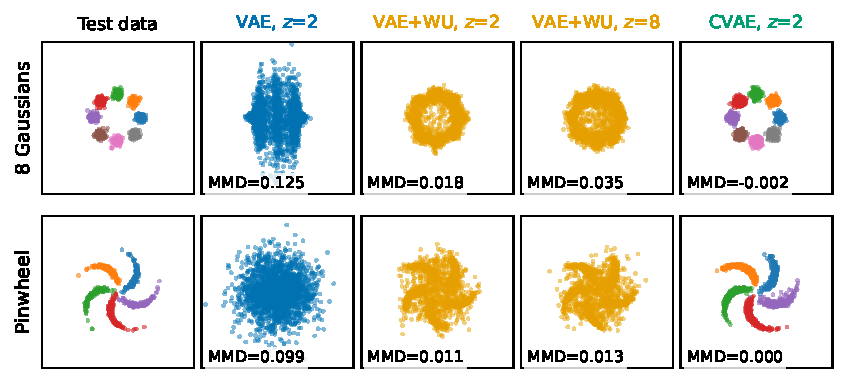
\includegraphics[width=\linewidth]{figures/report/toy_samples.pdf}
  \caption{Test data and 2{,}000 model samples (seed 0, MMD$^2$ inset).
  The plain VAE collapses to a single Gaussian blob; with KL warm-up (WU)
  it recovers the ring and the spiral but blurs the modes; the CVAE is
  almost exact. Colors are class labels (CVAE samples use their condition).}
  \label{fig:toy-samples}
\end{figure}

\begin{figure}[htbp]
  \centering
  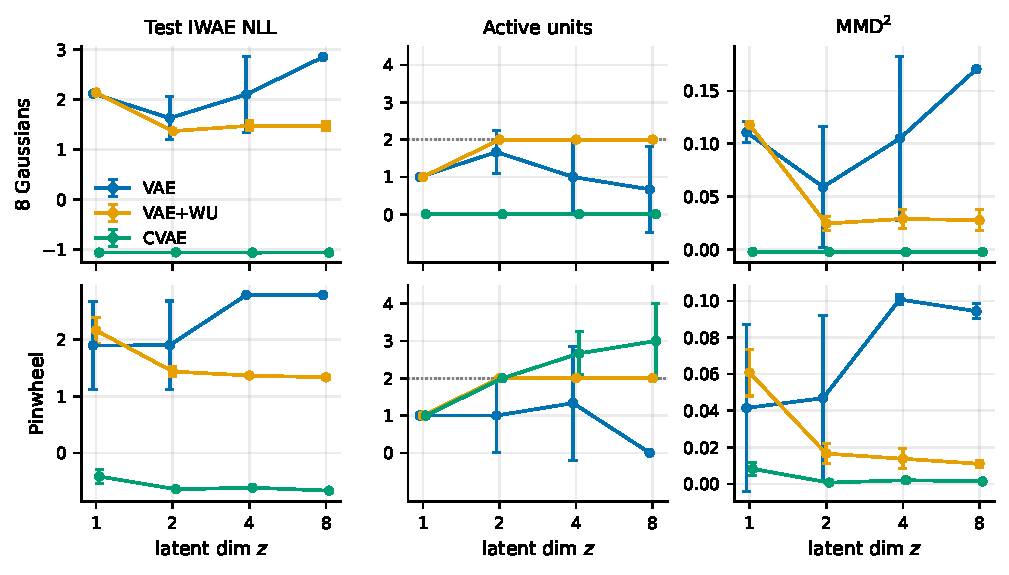
\includegraphics[width=\linewidth]{figures/report/toy_latent_sweep.pdf}
  \caption{Effect of latent size $d_z$ on the 2D data (mean $\pm$ std over
  three seeds): test IWAE NLL, active units, and sample MMD$^2$. With
  warm-up, the number of active units saturates at 2, the data
  dimension, for every $d_z\ge2$.}
  \label{fig:toy-sweep}
\end{figure}

\begin{table}[htbp]
  \centering
  \caption{2D results (standardized space; nats). VAE+WU = VAE with KL
  warm-up. Lower is better for all columns except AU.}
  \label{tab:toy}
  \footnotesize
  \setlength{\tabcolsep}{4pt}
  \begin{tabular}{llrcccccc}
\toprule
Dataset & Model & $z$ & Train $-$ELBO & Test $-$ELBO & Test IWAE NLL & KL & AU & MMD$^2$ \\
\midrule
8 Gaussians & VAE & 1 & $2.194\pm0.023$ & $2.178\pm0.029$ & $2.112\pm0.012$ & $1.85\pm0.04$ & $1.0\pm0.0$ & $0.111\pm0.010$ \\
 & VAE & 2 & $1.773\pm0.375$ & $1.813\pm0.384$ & $1.622\pm0.434$ & $2.48\pm0.50$ & $1.7\pm0.6$ & $0.059\pm0.057$ \\
 & VAE & 4 & $2.190\pm0.656$ & $2.246\pm0.623$ & $2.096\pm0.763$ & $1.69\pm1.58$ & $1.0\pm1.0$ & $0.105\pm0.078$ \\
 & VAE & 8 & $2.839\pm0.002$ & $2.839\pm0.004$ & $2.842\pm0.001$ & $0.01\pm0.01$ & $0.7\pm1.2$ & $0.171\pm0.002$ \\
\cmidrule{2-9}
 & VAE+WU & 1 & $2.189\pm0.015$ & $2.220\pm0.029$ & $2.133\pm0.006$ & $2.16\pm0.02$ & $1.0\pm0.0$ & $0.118\pm0.003$ \\
 & VAE+WU & 2 & $1.563\pm0.019$ & $1.573\pm0.029$ & $1.362\pm0.019$ & $3.27\pm0.06$ & $2.0\pm0.0$ & $0.024\pm0.006$ \\
 & VAE+WU & 4 & $1.687\pm0.108$ & $1.751\pm0.099$ & $1.470\pm0.097$ & $3.11\pm0.18$ & $2.0\pm0.0$ & $0.029\pm0.009$ \\
 & VAE+WU & 8 & $1.688\pm0.034$ & $1.714\pm0.058$ & $1.465\pm0.084$ & $3.01\pm0.14$ & $2.0\pm0.0$ & $0.028\pm0.010$ \\
\cmidrule{2-9}
 & CVAE & 1 & $-1.078\pm0.006$ & $-1.059\pm0.004$ & $-1.067\pm0.005$ & $0.00\pm0.00$ & $0.0\pm0.0$ & $-0.003\pm0.001$ \\
 & CVAE & 2 & $-1.068\pm0.011$ & $-1.046\pm0.026$ & $-1.061\pm0.011$ & $0.00\pm0.00$ & $0.0\pm0.0$ & $-0.002\pm0.001$ \\
 & CVAE & 4 & $-1.066\pm0.009$ & $-1.048\pm0.002$ & $\mathbf{-1.068\pm0.003}$ & $0.00\pm0.00$ & $0.0\pm0.0$ & $-0.003\pm0.001$ \\
 & CVAE & 8 & $-1.045\pm0.013$ & $-1.028\pm0.008$ & $-1.066\pm0.001$ & $0.00\pm0.00$ & $0.0\pm0.0$ & $-0.003\pm0.001$ \\
\midrule
Pinwheel & VAE & 1 & $2.065\pm0.672$ & $2.007\pm0.673$ & $1.895\pm0.770$ & $1.77\pm1.53$ & $1.0\pm0.0$ & $0.041\pm0.046$ \\
 & VAE & 2 & $2.058\pm0.690$ & $2.054\pm0.644$ & $1.900\pm0.779$ & $2.09\pm1.87$ & $1.0\pm1.0$ & $0.047\pm0.045$ \\
 & VAE & 4 & $2.839\pm0.002$ & $2.788\pm0.005$ & $2.786\pm0.001$ & $0.02\pm0.02$ & $1.3\pm1.5$ & $0.101\pm0.003$ \\
 & VAE & 8 & $2.841\pm0.002$ & $2.789\pm0.006$ & $2.785\pm0.000$ & $0.01\pm0.01$ & $0.0\pm0.0$ & $0.094\pm0.004$ \\
\cmidrule{2-9}
 & VAE+WU & 1 & $2.191\pm0.250$ & $2.277\pm0.152$ & $2.162\pm0.226$ & $2.57\pm0.19$ & $1.0\pm0.0$ & $0.061\pm0.013$ \\
 & VAE+WU & 2 & $1.715\pm0.108$ & $1.699\pm0.025$ & $1.436\pm0.083$ & $3.79\pm0.15$ & $2.0\pm0.0$ & $0.017\pm0.005$ \\
 & VAE+WU & 4 & $1.680\pm0.070$ & $1.656\pm0.028$ & $1.366\pm0.016$ & $3.72\pm0.04$ & $2.0\pm0.0$ & $0.014\pm0.005$ \\
 & VAE+WU & 8 & $1.637\pm0.051$ & $1.597\pm0.048$ & $1.334\pm0.029$ & $3.70\pm0.04$ & $2.0\pm0.0$ & $0.011\pm0.002$ \\
\cmidrule{2-9}
 & CVAE & 1 & $-0.361\pm0.162$ & $-0.352\pm0.141$ & $-0.412\pm0.122$ & $1.37\pm0.22$ & $1.0\pm0.0$ & $0.008\pm0.004$ \\
 & CVAE & 2 & $-0.547\pm0.036$ & $-0.520\pm0.044$ & $-0.637\pm0.009$ & $1.85\pm0.06$ & $2.0\pm0.0$ & $0.001\pm0.000$ \\
 & CVAE & 4 & $-0.495\pm0.053$ & $-0.522\pm0.039$ & $-0.610\pm0.025$ & $1.76\pm0.10$ & $2.7\pm0.6$ & $0.002\pm0.001$ \\
 & CVAE & 8 & $-0.578\pm0.032$ & $-0.579\pm0.026$ & $\mathbf{-0.662\pm0.015}$ & $1.88\pm0.03$ & $3.0\pm1.0$ & $0.001\pm0.001$ \\
\bottomrule
\end{tabular}

\end{table}

\paragraph{Posterior collapse grows with latent size.}
Without warm-up, the unconditional VAE often converges to a degenerate
solution: every latent dimension has KL $\approx0$, the decoder ignores
$z$, and the model is a single Gaussian ($-$ELBO $\approx2.84$, the same
for both datasets; Figure~\ref{fig:toy-samples}, second column). With a
Gaussian decoder whose variance is learned, this solution is a stable
local optimum: early in training the KL term is cheap to remove, while the
reconstruction benefit of using $z$ appears only after the decoder has
learned to use it. Collapse becomes \emph{more} likely with a larger
latent space: at $d_z=8$ (and already at $d_z=4$ on pinwheel) all three
seeds collapse, while at smaller $d_z$ some seeds escape (hence the huge error bars in
Table~\ref{tab:toy}). A larger latent space therefore made the plain VAE
\emph{worse}, not merely wasteful.

\paragraph{With warm-up, extra dimensions are switched off.}
KL warm-up removes the collapse (Figure~\ref{fig:toy-sweep}). For every
$d_z\ge2$ exactly two units are active, the intrinsic dimension of the
data, and the remaining dimensions have KL $\approx0$ (per-dimension KL in
Figure~\ref{fig:toy-kldims}). Test NLL and MMD$^2$ are then nearly flat in
$d_z$, so beyond the data dimension a larger latent space neither helps nor
hurts. $d_z=1$ is too small on both datasets (NLL $2.1$ vs.\ $1.4$).
Both distributions are approximately one-dimensional curves, a ring and
five arms, but a continuous decoder maps the connected Gaussian prior to a
connected set; it must either cut the ring or draw a trail of
low-density samples between arms, and the 2D latent avoids this. Even the
best unconditional VAE blurs the modes (Figure~\ref{fig:toy-samples}):
the Gaussian prior puts mass in the gaps between clusters, and those
regions decode to points between clusters.

\paragraph{Conditioning removes the need for a latent code.}
The CVAE is far better on both datasets (NLL $-1.07$ vs.\ $1.36$ on 8
Gaussians, $-0.66$ vs.\ $1.33$ on pinwheel) and its samples match the data
(MMD$^2\approx0$). On 8 Gaussians it uses \emph{zero} latent dimensions at
every $d_z$: given the label, each cluster is an isotropic Gaussian that
the decoder's mean and variance already describe exactly, so any KL spent
on $z$ is wasted. On pinwheel each arm is curved, so the CVAE uses about
two dimensions to place a point along and across the arm; AU grows
slightly with $d_z$ (2, 2.7, 3 for $d_z=2,4,8$), but the extra units carry
little KL and do not change the NLL. Conditioning thus moves information
from $z$ into $c$: the latent space only has to encode the variation
\emph{within} a class.

\paragraph{Architecture.} For the pinwheel CVAE ($d_z=2$), width matters
more than depth: test NLL improves from $-0.44$ to $-0.52$ with 32 units
and to about $-0.65$ with 128--512 units, with little change across 1--3
hidden layers.

\begin{figure}[htbp]
  \centering
  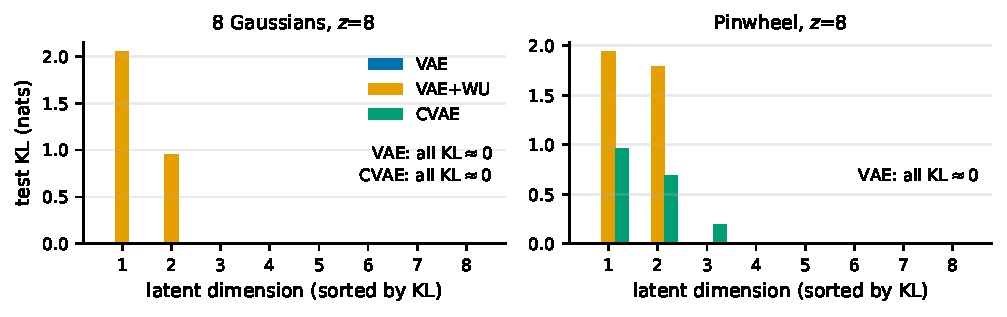
\includegraphics[width=\linewidth]{figures/report/toy_kl_dims.pdf}
  \caption{Per-dimension test KL for $d_z=8$ (seed 0), sorted. Only two
  dimensions are used by the VAE with warm-up; the plain VAE uses none.}
  \label{fig:toy-kldims}
\end{figure}

% ============================================================
\section{MNIST Experiments}
We trained 40 models. The latent sweep uses a CVAE (MLP, $h=512$, $L=2$)
with $d_z\in\{2,4,8,16,32,64\}$ and three seeds, plus the same unconditional
VAE with one seed. The architecture sweep (CVAE, $d_z=16$) varies width
$\{256,512\}$ and depth $\{1,2,3\}$ and adds the convolutional model, with two
seeds each. The optimization sweep changes the learning rate or the batch
size of the baseline. No MNIST run collapsed without warm-up: every model has
at least five active units.

\begin{figure}[htbp]
  \centering
  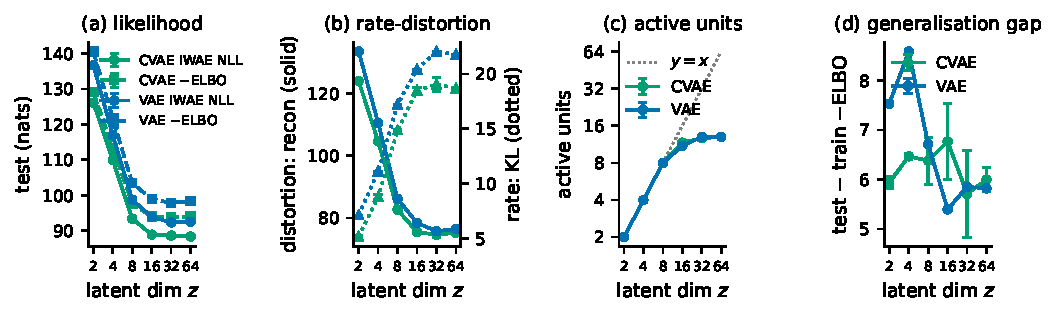
\includegraphics[width=\linewidth]{figures/report/mnist_latent_sweep.pdf}
  \caption{MNIST latent sweep (CVAE: mean $\pm$ std over three seeds; VAE:
  one seed). (a) Test IWAE NLL (solid) and $-$ELBO (dashed). (b) Distortion
  (reconstruction NLL, solid, left axis) and rate (KL, dotted, right axis).
  (c) Active units; the dotted line is $\text{AU}=d_z$. (d) Gap between test
  and train $-$ELBO.}
  \label{fig:mnist-sweep}
\end{figure}

\begin{table}[htbp]
  \centering
  \caption{MNIST latent sweep (test set, nats). The CVAE NLL is
  $-\log p(x\mid c)$; add $H(c)=2.30$ to compare it with the VAE. FID is
  computed in our classifier's feature space (train-vs-test floor 3.4). Acc
  is the fraction of CVAE samples classified as their requested label.}
  \label{tab:mnist-latent}
  \footnotesize
  \setlength{\tabcolsep}{3.5pt}
  \begin{tabular}{llrrrrrrrr}
\toprule
Model & $z$ & Train $-$ELBO & Test $-$ELBO & Test IWAE & Recon & KL & AU & FID & Acc (\%) \\
\midrule
CVAE & 2 & 123.1 $\pm$ 0.1 & 129.1 $\pm$ 0.2 & 126.0 $\pm$ 0.1 & 123.9 $\pm$ 0.1 & 5.2 $\pm$ 0.1 & 2.0 $\pm$ 0.0 & 198.4 $\pm$ 5.4 & 98.2 $\pm$ 0.2 \\
CVAE & 4 & 106.9 $\pm$ 0.2 & 113.4 $\pm$ 0.2 & 109.9 $\pm$ 0.2 & 104.6 $\pm$ 0.3 & 8.8 $\pm$ 0.2 & 4.0 $\pm$ 0.0 & 116.9 $\pm$ 6.2 & 97.1 $\pm$ 0.3 \\
CVAE & 8 & 91.2 $\pm$ 0.4 & 97.6 $\pm$ 0.1 & 93.4 $\pm$ 0.0 & 82.7 $\pm$ 0.1 & 14.9 $\pm$ 0.1 & 8.0 $\pm$ 0.0 & 63.0 $\pm$ 4.2 & 94.8 $\pm$ 0.4 \\
CVAE & 16 & 87.2 $\pm$ 0.8 & 94.0 $\pm$ 0.2 & 88.9 $\pm$ 0.4 & 75.5 $\pm$ 0.4 & 18.5 $\pm$ 0.3 & 11.7 $\pm$ 0.6 & 57.6 $\pm$ 3.1 & 93.9 $\pm$ 0.1 \\
CVAE & 32 & 88.1 $\pm$ 1.0 & 93.8 $\pm$ 0.2 & 88.6 $\pm$ 0.4 & 74.7 $\pm$ 0.8 & 19.1 $\pm$ 0.6 & 12.7 $\pm$ 0.6 & 72.8 $\pm$ 10.6 & 92.5 $\pm$ 0.2 \\
CVAE & 64 & 88.0 $\pm$ 0.3 & 94.0 $\pm$ 0.1 & \textbf{88.4 $\pm$ 0.2} & 75.3 $\pm$ 0.0 & 18.7 $\pm$ 0.1 & 13.0 $\pm$ 0.0 & 65.7 $\pm$ 3.3 & 93.3 $\pm$ 0.4 \\
\midrule
VAE & 2 & 133.0 & 140.6 & 136.7 & 133.4 & 7.1 & 2.0 & 360.6 & -- \\
VAE & 4 & 113.0 & 121.6 & 116.9 & 110.5 & 11.1 & 4.0 & 211.7 & -- \\
VAE & 8 & 96.7 & 103.4 & 98.7 & 86.2 & 17.2 & 8.0 & 190.0 & -- \\
VAE & 16 & 93.5 & 98.9 & 93.9 & 78.4 & 20.4 & 11.0 & 177.7 & -- \\
VAE & 32 & 92.0 & 97.9 & 92.3 & 75.8 & 22.1 & 13.0 & 178.8 & -- \\
VAE & 64 & 92.5 & 98.3 & 92.5 & 76.5 & 21.8 & 13.0 & 191.7 & -- \\
\bottomrule
\end{tabular}

\end{table}

\paragraph{Likelihood saturates near 16 latent dimensions.}
For $d_z\le8$, every latent dimension is active, and each doubling of $d_z$
buys a large improvement: test NLL goes from $126.0$ to $109.9$ to $93.4$
nats (Table~\ref{tab:mnist-latent}). The model trades rate for distortion:
the KL rises from $5.2$ to $14.9$ nats while the reconstruction term falls
from $123.9$ to $82.7$ (Figure~\ref{fig:mnist-sweep}b). Beyond $d_z=16$
the curves flatten. The NLL is $88.9$, $88.6$ and $88.4$ for $d_z=16,32,64$,
and both rate and distortion stay constant. The number of active units
saturates at 12--13 (Figure~\ref{fig:mnist-sweep}c), so at $d_z=64$ about 51
dimensions have KL $\approx0$. This is the MNIST analogue of the 2D result:
the ELBO switches off dimensions it does not need. The saturation point, not
$d_z$, measures how much latent structure the model can exploit. The
train--test gap (5--9 nats) does not grow with $d_z$
(Figure~\ref{fig:mnist-sweep}d), because the switched-off dimensions add no
capacity. Validation $-$ELBO bottoms out after 35--50 epochs, and early
stopping caps the overfitting.

\paragraph{The label replaces about $\ln 10$ nats of code.}
The unconditional VAE spends $1.9$--$3.1$ nats more KL than the CVAE at
every $d_z$, close to the $2.30$ nats needed to encode which digit it is.
After adding $H(c)$ to the CVAE's NLL, the CVAE is still better: by $8.3$
nats at $d_z=2$, $3.0$ at $d_z=8$, and $1.4$--$1.9$ at $d_z\ge32$. The
benefit of conditioning is therefore largest when the latent space is small.
A 2D latent must spend its capacity on class identity.
Figure~\ref{fig:mnist-manifold} shows this. The $d_z=2$ VAE manifold is a
map of digit classes, and the transitions between classes pass through
ambiguous shapes. The CVAE's two dimensions instead encode style: $z_1$
roughly controls slant and $z_2$ width and stroke thickness, along similar
axes for 3s and 8s. The style-swap experiment
(Figure~\ref{fig:mnist-swap}) confirms that the code is largely
label-independent. An image encoded with its true label and decoded with
the other nine labels keeps its slant and thickness. At $d_z=16$,
reconstructions are sharp but a few swaps break (e.g.\ a 7 drawn in the
style of a 2). Some dimensions therefore carry class-specific shape, which
the 2D code is too small to hold.

\begin{figure}[htbp]
  \centering
  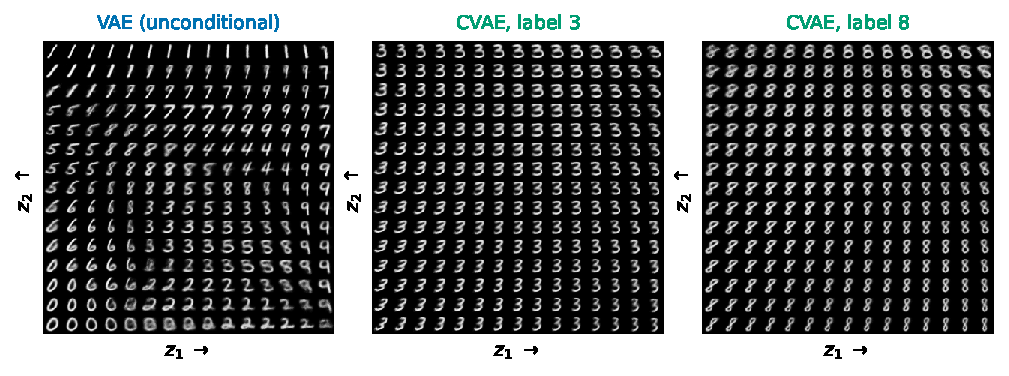
\includegraphics[width=0.85\linewidth]{figures/report/mnist_manifold.pdf}
  \caption{Decoder means over a $15\times15$ grid of $z$ for $d_z=2$
  (seed 0). The unconditional VAE organizes $z$ by digit class; the CVAE uses
  $z$ for style, along similar directions for both labels.}
  \label{fig:mnist-manifold}
\end{figure}

\begin{figure}[htbp]
  \centering
  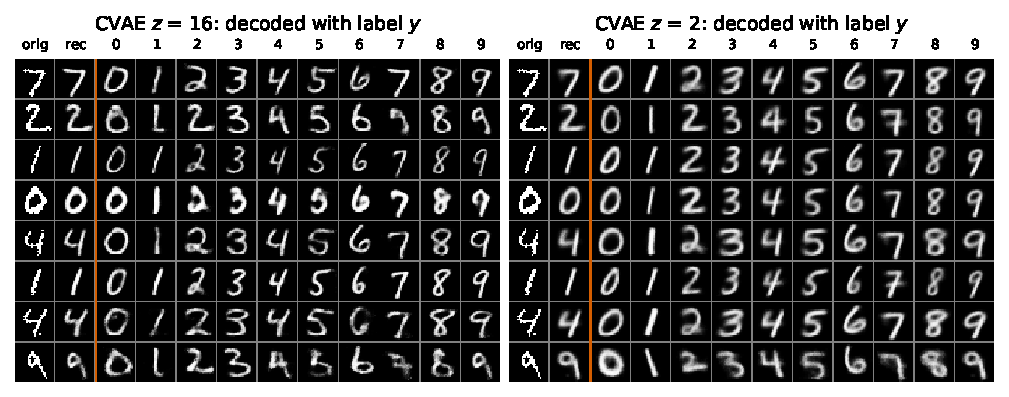
\includegraphics[width=0.9\linewidth]{figures/report/mnist_style_swap.pdf}
  \caption{Style swap. A test image (orig) is encoded with its label,
  reconstructed (rec), and decoded with each of the ten labels.}
  \label{fig:mnist-swap}
\end{figure}

\paragraph{Sample quality does not follow likelihood.}
Figure~\ref{fig:mnist-samples} and Figure~\ref{fig:mnist-quality} examine
samples $x\sim p_\theta(x\mid z,c)$, $z\sim\mathcal N(0,I)$. With $d_z=2$,
the CVAE's samples are recognizable (98.2\% are classified as the requested
digit) but nearly identical within a class: each row of the grid is one
blurry prototype, and its FID is high ($198$). Increasing $d_z$ to 8--16
adds diversity and detail, and FID falls to $58$--$63$. Past that point FID
rises again ($73$ and $66$ at $d_z=32,64$, with large seed variance), and
label accuracy keeps falling to about 93\%: more samples have broken strokes
or look like another digit, although the NLL still improves slightly. One
explanation consistent with this is that the aggregate posterior
$q(z)=\mathbb E_x\,q(z\mid x)$ fills the prior less evenly as the number of
active dimensions grows. Prior samples then land in regions the decoder
rarely saw during training. The mismatch is not in the first two moments: a
Gaussian fitted to $q(z)$ is within $0.15$ nats of $\mathcal N(0,I)$ for
every run. Any mismatch must therefore lie in the shape of $q(z)$. The
unconditional VAE's FID is about $180$--$190$ for all $d_z\ge8$, three times
the CVAE's. Its samples include ambiguous digits from the regions between
class clusters, the same mode-blurring seen in 2D, and its class
proportions are slightly unbalanced (entropy of predicted classes below
$\ln10$).

\begin{figure}[htbp]
  \centering
  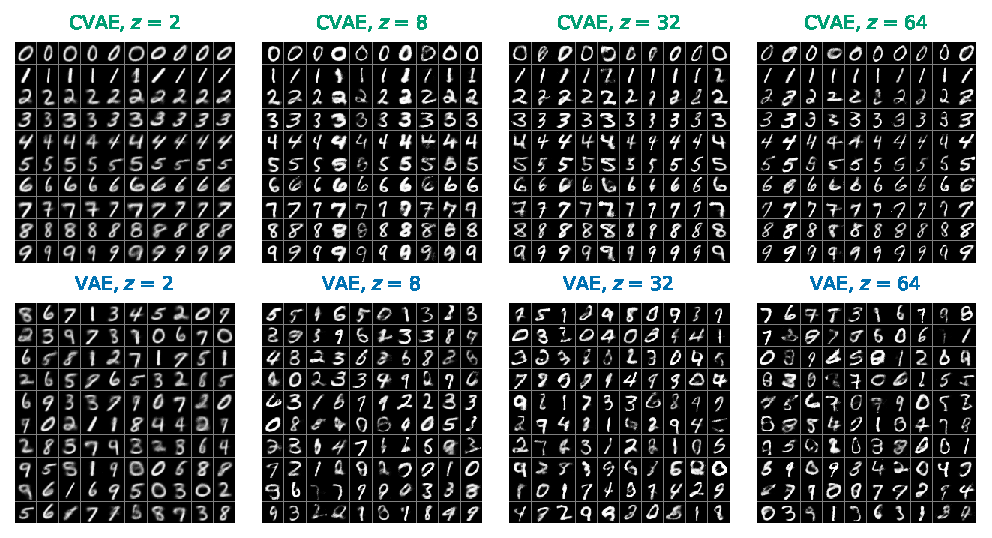
\includegraphics[width=0.85\linewidth]{figures/report/mnist_samples_by_z.pdf}
  \caption{Random samples (decoder means, seed 0). CVAE rows are labels
  $0$--$9$, and each column shares the same $z$. Small $d_z$ gives clean but
  prototypical digits; large $d_z$ gives diverse digits with more defects.}
  \label{fig:mnist-samples}
\end{figure}

\begin{figure}[htbp]
  \centering
  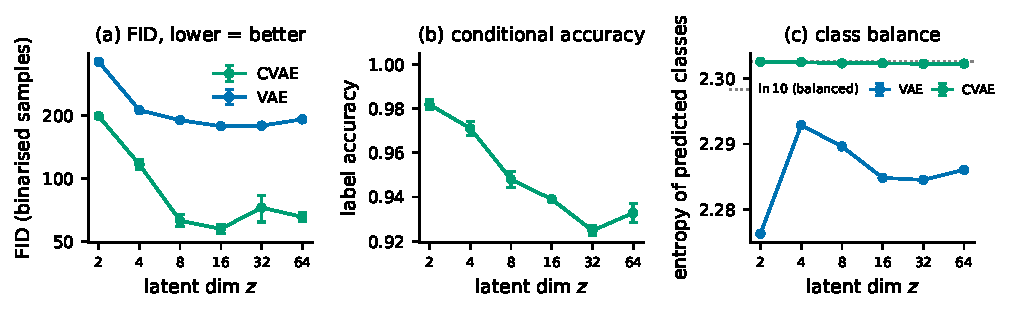
\includegraphics[width=\linewidth]{figures/report/mnist_sample_quality.pdf}
  \caption{Sample quality versus $d_z$ (10k samples per model). (a) FID in
  classifier-feature space (log scale). (b) Fraction of CVAE samples
  classified as the requested label. (c) Entropy of the predicted-class
  histogram; $\ln10$ means perfectly balanced classes.}
  \label{fig:mnist-quality}
\end{figure}

\begin{table}[htbp]
  \centering
  \caption{MNIST architecture sweep (CVAE, $d_z=16$, two seeds).
  Gap = test $-$ train $-$ELBO. Training is capped at 100 epochs.}
  \label{tab:mnist-arch}
  \footnotesize
  \setlength{\tabcolsep}{3.5pt}
  \begin{tabular}{lrrrrrrrr}
\toprule
Architecture & \#params & Test IWAE & Test $-$ELBO & Gap & AU & FID & Best ep. & Time (min) \\
\midrule
MLP $h$=256, $d$=1 & 0.42M & 91.4 $\pm$ 0.1 & 96.2 $\pm$ 0.1 & 2.5 $\pm$ 0.1 & 16.0 $\pm$ 0.0 & 158.1 $\pm$ 6.7 & 90 $\pm$ 6 & 1.3 $\pm$ 0.1 \\
MLP $h$=256, $d$=2 & 0.55M & 89.3 $\pm$ 0.9 & 94.2 $\pm$ 0.7 & 4.7 $\pm$ 0.3 & 12.0 $\pm$ 1.4 & 61.2 $\pm$ 0.6 & 82 $\pm$ 21 & 1.3 $\pm$ 0.2 \\
MLP $h$=256, $d$=3 & 0.68M & 103.4 $\pm$ 0.1 & 107.3 $\pm$ 0.1 & 6.0 $\pm$ 0.2 & 5.0 $\pm$ 0.0 & 76.1 $\pm$ 7.3 & 60 $\pm$ 3 & 1.2 $\pm$ 0.0 \\
MLP $h$=512, $d$=1 & 0.84M & 90.3 $\pm$ 0.2 & 95.3 $\pm$ 0.0 & 4.4 $\pm$ 0.5 & 16.0 $\pm$ 0.0 & 135.4 $\pm$ 11.4 & 79 $\pm$ 20 & 1.6 $\pm$ 0.2 \\
MLP $h$=512, $d$=2 (base) & 1.36M & 88.7 $\pm$ 0.0 & 93.9 $\pm$ 0.0 & 6.9 $\pm$ 1.0 & 12.0 $\pm$ 0.0 & 58.5 $\pm$ 3.8 & 50 $\pm$ 12 & 1.5 $\pm$ 0.2 \\
MLP $h$=512, $d$=3 & 1.89M & 99.1 $\pm$ 0.2 & 103.3 $\pm$ 0.1 & 6.2 $\pm$ 1.1 & 6.0 $\pm$ 0.0 & 60.1 $\pm$ 5.3 & 30 $\pm$ 8 & 1.4 $\pm$ 0.2 \\
Conv & 3.32M & 84.4 $\pm$ 0.9 & 89.2 $\pm$ 0.7 & 4.5 $\pm$ 0.5 & 14.5 $\pm$ 2.1 & 37.7 $\pm$ 3.7 & 46 $\pm$ 5 & 5.6 $\pm$ 0.5 \\
\bottomrule
\end{tabular}

\end{table}

\paragraph{Architecture: depth trades rate for likelihood.}
The convolutional model has the best likelihood and samples (NLL $84.4$,
FID $37.7$; Table~\ref{tab:mnist-arch}): its inductive bias for images
helps more than extra width. Among MLPs, $512$ units beat $256$ at each
depth by $0.6$--$4$ nats. Depth shows two failure modes in opposite
directions. With one hidden layer, the model uses all 16 dimensions and has
the highest rate ($21.6$ nats). It is still improving at the 100-epoch limit
(best epoch 64--94), and its NLL is only $1.6$--$2.7$ nats worse than the
baseline, yet its samples are the worst (FID $135$--$158$, 87--89\%
accuracy). With three hidden layers, NLL degrades by $10$--$14$ nats while
AU drops to 5--6 and the rate to $10$--$12$ nats. This is a partial posterior
collapse: the deeper decoder relies on the label and a few dimensions.
Training stops early (epochs 30--60). Its samples are nevertheless the most
recognizable (98\% accuracy) and have an FID close to the baseline
($60$--$76$), because they are low-diversity prototypes.

\paragraph{Optimization.} With one seed per setting (seed spread at the
baseline: $0.4$ nats), learning rate matters most. A learning rate of
$3\times10^{-4}$ gives the best MLP NLL ($87.4$ vs.\ $88.7$) but needs 89
epochs. $3\times10^{-3}$ ends at a lower-rate solution (KL $15.2$, AU 9) and
NLL $94.8$, a mild form of the same collapse. Batch size $256$ is on par with
$128$ ($88.3$), and $64$ is slightly worse ($90.0$).

% ============================================================
\section{Discussion and Conclusion}

\paragraph{Choosing the latent size.} On both 2D and MNIST data, we see
three regimes. Below the data's usable dimensionality ($d_z=1$ in 2D,
$d_z\le8$ on MNIST), every dimension is active, the model is
rate-limited, and samples are blurry prototypes. In a middle range
($d_z\approx2$ in 2D, 8--16 on MNIST), likelihood is near its best and
sample quality is best. Beyond it, the ELBO switches off the extra
dimensions: AU saturates at 2 in 2D and at 12--13 on MNIST, and
likelihood is flat. On MNIST the larger latent spaces still produced
slightly worse samples. A practical rule is to choose $d_z$ just above the
point where active units saturate and to judge sample quality directly,
since NLL does not detect its decline.

\paragraph{Why collapse depends on the decoder.} The plain VAE collapsed on
the 2D data but never on MNIST. In 2D, a Gaussian decoder with learned
variance can fit the data reasonably well without $z$. Collapsing costs
only about $1.4$ nats ($2.84$ vs.\ $1.3$--$1.5$), so the optimizer has
little incentive to leave the collapsed solution, especially when the KL
penalty is spread over many dimensions. On MNIST, a decoder that ignores
$z$ scores $206$ nats (independent Bernoulli pixels), more than 100 nats
worse than the VAE, so using $z$ always pays. The partial collapse of the
3-layer MLP and the high-learning-rate run shows that optimization can still
reach low-rate solutions when the decoder is flexible. KL warm-up, which
fixed the 2D case, is the natural remedy; we did not test it on MNIST.

\paragraph{Conditioning.} Giving the model the label moves information out
of $z$. That information is about $\ln10$ nats on MNIST, the whole cluster
identity on 8 Gaussians. The latent space then only has to encode
within-class variation, which is smaller, smoother, and shared across
classes (style swap). Conditioning improved likelihood and especially
sample quality (FID $58$ vs.\ $178$ at $d_z=16$), and the gain was largest
for small latent spaces.

\paragraph{Likelihood is not sample quality.} Three comparisons show that
held-out likelihood and sample quality can disagree:
$d_z=64$ vs.\ $16$ (better NLL, worse samples), depth 1 vs.\ 2
(similar NLL, much worse samples), and depth 3 (much worse NLL,
recognizable samples). The ELBO rewards explaining every test image. It does
not penalize prior regions that decode to poor images, nor reward diversity
directly. Evaluating a VAE therefore requires looking at samples, not only
at test error.

\paragraph{Limitations.} The unconditional VAE and the optimization sweep
use one seed. Our FID uses features from our own classifier and is only
comparable within this study. Training was capped at 100 epochs, which
affects the 1-layer MLPs and the low-learning-rate run. The moment-matching
test of $q(z)$ cannot detect non-Gaussian holes, so the prior-hole
explanation remains a hypothesis.

\paragraph{Use of generative AI.}
Generative AI tools supported implementation of the training and analysis
code from detailed author plans. They also improved the report's
organization, formatting, wording, figures, and tables.

\begin{thebibliography}{9}\small
\bibitem{kingma2014} D.~P. Kingma and M.~Welling. Auto-encoding variational
  Bayes. \emph{ICLR}, 2014.
\bibitem{sohn2015} K.~Sohn, H.~Lee, and X.~Yan. Learning structured output
  representation using deep conditional generative models. \emph{NeurIPS},
  2015.
\bibitem{bowman2016} S.~R. Bowman et al. Generating sentences from a
  continuous space. \emph{CoNLL}, 2016.
\bibitem{burda2016} Y.~Burda, R.~Grosse, and R.~Salakhutdinov. Importance
  weighted autoencoders. \emph{ICLR}, 2016.
\bibitem{johnson2016} M.~J. Johnson et al. Composing graphical models with
  neural networks for structured representations and fast inference.
  \emph{NeurIPS}, 2016.
\end{thebibliography}

\end{document}
